%% LyX 1.6.7 created this file.  For more info, see http://www.lyx.org/.
%% Do not edit unless you really know what you are doing.
\documentclass[twocolumn,english,british]{IEEEtran}
\renewcommand{\sfdefault}{lmss}
\renewcommand{\familydefault}{\sfdefault}
\usepackage[T1]{fontenc}
\usepackage{babel}

\usepackage{verbatim}
\usepackage{float}
\usepackage{pdfpages}
\usepackage[dot]{bibtopic}
\usepackage[unicode=true, 
 bookmarks=true,bookmarksnumbered=false,bookmarksopen=false,
 breaklinks=false,pdfborder={0 0 0},backref=false,colorlinks=false]
 {hyperref}
\hypersetup{pdftitle={DHT based Nat  traversal},
 pdfauthor={David Irvine},
 pdfsubject={Networking},
 pdfkeywords={PKI, DHT, Security }}

\makeatletter

%%%%%%%%%%%%%%%%%%%%%%%%%%%%%% LyX specific LaTeX commands.
\providecommand{\LyX}{L\kern-.1667em\lower.25em\hbox{Y}\kern-.125emX\@}
%% A simple dot to overcome graphicx limitations
\newcommand{\lyxdot}{.}

\floatstyle{ruled}
\newfloat{algorithm}{tbp}{loa}
\floatname{algorithm}{Algorithm}

%%%%%%%%%%%%%%%%%%%%%%%%%%%%%% Textclass specific LaTeX commands.
\newcommand{\lyxrightaddress}[1]{
\par {\raggedleft \begin{tabular}{l}\ignorespaces
#1
\end{tabular}
\vspace{1.4em}
\par}
}
% protect \markboth against an old bug reintroduced in babel >= 3.8g
\let\oldforeign@language\foreign@language
\DeclareRobustCommand{\foreign@language}[1]{%
  \lowercase{\oldforeign@language{#1}}}

\makeatother

\begin{document}

\title{DHT based NAT traversal}


\author{David Irvine, email: david.irvine@maidsafe.net, LifeStuff David}

\maketitle

\lyxrightaddress{maidsafe.net limited (registered in Scotland Sc 297540)}

September, 2010
\begin{abstract}
Today's Distributed Hash Tables (DHT's) and other overlay networks
are based on operating without hindrance of real world issues regarding
connectivity between nodes. This is not a problem when operating in
a private or controlled environment, but in the transition to peer
to peer or fully distributed networks, it becomes a major headache.
This paper introduces a pure p2p solution to Network Address Translation
(NAT) traversal, which is probably the main problem facing public
p2p networks.\end{abstract}
\begin{IEEEkeywords}
security, freedom, privacy, DHT, encryption
\end{IEEEkeywords}

\markboth{maidsafe.net limited company confidential Version 0.1}{...}

\tableofcontents{}

\listoftables





\section{Introduction}

\PARstart{I}{nternet} technology allows the interconnect of every
device to every other device, in principle. In practice, this is not
the case and for many reasons devices tend to be behind routers that
allow them to go unnoticed or at least act as a proxy device. This
helps connect multiple devices to a single publicly addressable IP
location. The devices behind the router may have private or classified
private addresses and number in thousands all connected to the Internet
and appearing as one single identity. The router will proxy requests
and responses in many cases to hide the devices. 

NAT is a good solution for the lack of publicly available IP addresses
with the current incumbent scheme of IP version 4, IP version 6 will
allow more than enough public addresses to exist and in fact provide
several addresses for every square meter of the planet. Even with
IP6, however there will still be NAT devices around and NAT traversal
will still be required.

Several methods exist for traversing NAT devices, including \emph{Session
Traversal Utilities for NAT (STUN) \cite{1} }which is extended to
form\emph{ Interactive Connectivity Establishment (ICE): A Protocol
for Network Address Translator (NAT) Traversal for Offer/Answer Protocols
}\cite{2}. This paper will present a mechanism to exploit these technologies
without the requirement for any servers to exist. This is therefore
a solution for distributed protocols that in fact requires a distributed
protocol to exist (a good fit).


\section{NAT traversal methods}


\subsection{Router negotiation protocols}


\subsubsection{Universal Plug and Play (UPnP)\cite{5}}

UPnP is a UDT NAT traversal protocol which utilises HTTP over UDP
to negotiate a port mapping with an enabled router. This allows a
node to appear as though it has a directly connected IP (that of the
router) and port combination. From this perspective the node appears
directly connected (for that port). 

UPnP is seen as a security risk by many vendors and is supplied on
a routing device switched off. 

Care should be taken with the protocol to ensure that a permanent
mapping is requested, which would last until requested to be un-mapped
or the router is rebooted. The more effective solution is to select
a mapping for a period and refresh this every few seconds, to ensure
the router device is not congested with stale mappings. 

Many routers will have a low limit of concurrent available UPnP mappings.


\subsubsection{Network Address Translation Port Mapping Protocol (NAT-PMP)}

NAT-PMP is an upgrade of UPnP to attempt to alleviate the security
issues surrounding UPnP, it is currently not provided in many routers,
although this may change in the future. Again this is a UDP controlled
protocol and as such will not operate in networks that have banned
UDP. 


\subsection{Hole Punching }

Hole punching can successfully traverse approximately 82\%\cite{6}of
NAT devices. It makes use of the fact that a router will leave a UDP
port mapped after sending data out. This is done whether the UDP packet
is successfully delivered or not. This is a necessity for a connectionless
protocol as the router cannot tell whether the transmission will be
successful or whether there is to be a reply (which all well defined
protocols using UDP should ensure there is).

The basis of the process is described in Algorithm 1, it is relatively
simple and uses this conversation method to operate. It should be
noted for BSD type socket API's it is important to ensure the SO\_REUSE\_ADDR
is set, allowing address reuse (very important). Using a UDP overlay
type protocol sch as UDT \cite{7} would introduce some new difficulties
here and the connection set-up time-out should be set very small,
as the first connection attempt will most likely fail, reducing time-outs
makes for more efficient code. 

%
\begin{algorithm}
\caption{Let A and B be the two hosts, each in its own private network; N1
and N2 are the two NAT devices; S is a public server with a well-known
globally reachable IP address. A and B each send a UDP packet to S;
the NAT devices N1 and N2 create UDP translation states and assign
temporary external port numbers S relays these port numbers back to
A and B A and B contact each others' NAT devices directly on the translated
ports; the NAT devices use the previously created translation states
and send the packets to A and B}

\end{algorithm}



\subsection{Relay nodes }

TURN is a system where a node will relay informations from a another
node behind an unfriendly NAT device. In this case fairness is a major
concern as the relay node will have to provide more bandwidth to the
fire-walled node. This cannot be handed off to alleviate the burden
which is unfortunate. Further research may prove to be very interesting
in these cases though. 


\section{NAT Traversal with a DHT}

Use of a DHT makes no difference to any router negotiation protocol
as described above, but can significantly improve the performance
and security of UDP hole punching techniques. 


\subsection{STUN server functionality in a DHT}

A STUN server, generally has 2 network interface cards on different
IP addresses (and preferably routes). This allows multiple routes
to a node to be confirmed in a manner similar to algorithm 1. In a
DHT, there should be no servers and in maidsafe\_dht all machines
should be able to be unknown in configuration terms, i.e. we cannot
presume we will have dual homed machines on the network. This initially
would appear to be a problem, whereas in fact it is an advantage.
In place of a dual homed server, a DHT has something more powerful,
a full network of nodes on different networks that can all message
each other and in many ways act like a huge server. Therefore, to
emulate a simple dual homes machine that exists on two networks is
perhaps one of the simplest tasks we can ask a DHT to perform. A DHT
performs these tasks efficiently and without exposing any server location
for an attack to be carried out. 

To achieve the STUN type functionality, we simply carry out the process
as defined in section \ref{sub:DHT-hole-punch}, where we use a node
on the network to perform NAT detection and traversal techniques.
This negates the requirement for a server, but, how do other clients
know which sever to speak to in case of a port restricted situation,
where the server requires a message to be sent and relayed to the
node we intended. Without this any port restricted node would be unreachable.
This is where we use a DHT component that provides us with such capability
and this is the routing table or list of contacts. 

In the contact tuple for each contact, where an intermediate node
is required (AKA STUN server) a node's address is stored along with
the end nodes address. So every node that requires an intermediate,
establishes the details of the intermediary and publishes this to
the network as part of its contact details. This is extremely effective
and simple to implement.


\subsection{DHT Hole Punching}

The process is very similar to non DHT hole punching, except that
for a network to be a pure distributed network there should be no
servers, therefore the STUN type server employed in a normal configuration
cannot be used. 


\subsection{DHT hole punch NAT traversal process\label{sub:DHT-hole-punch}}

Booststrap node = {[}B{]}; Our node = {[}U{]}, Other node who is not
sharing the same IP as {[}U{]} = {[}O{]}
\begin{enumerate}
\item On initial bootstrap, receive IP and port {[}B{]} detects.
\item If IP = a local IP then directly connected {[}stop{]}
\item Send Detection packet to {[}B{]} which in turn sends a packet to {[}O{]}. 
\item Both {[}B{]} and {[}O{]} send message to {[}U{]} and await reply.
\item If {[}O{]} receives a reply, it messages {[}B{]} with success. {[}B{]}
reports back to {[}U{]} that we are behind a full cone NAT. {[}stop{]}
\item If {[}O{]} cannot get a reply, it asks {[}B{]} to message {[}U{]}
with an attempt to connect to {[}O{]} (which may fail), at the same
time {[}O{]} tries to connect to {[}U{]}. If successful {[}O{]} reports
back to {[}B{]} with success, and is then behind a port restricted
NAT {[}stop{]}.
\item If 6. fails {[}U{]} is behind another type of NAT, probably symmetric,
although these is some success at predicting port increment or decrement
symmetric NAT devices, it is not efficient enough so {[}stop{]} with
fail at this point.
\end{enumerate}
On all attempts failing the node should report NAT traversal fail
to the application. This is not the final attempt as will be described
in \ref{sub:TCP-fallback-configuration}. 

This situation, however, should mean that a server node or an autonomous
network node should fail as the remaining options would be bandwidth
restrictive at this time to complete. 


\subsubsection{Implementation}

The above solution is purely hole punching, items 1 \& 2 should always
be tested first, on fail, then it is suggested three threads be created
and on one thread run the rest of this list to complete the hole punch
attempt. On threads 2 and 3 the router negotiations protocols should
be attempted (one on each thread). 

If 5 above passes then all thread should be stopped and the node will
start another thread to send keep alive messages to {[}B{]}, otherwise
UPnP or NAT-PMP will hopefully pass, it is advisable to accept a NAT-PMP
as first choice in this case. 


\subsection{Relay request}

In situations where all attempts to traverse a NAT fail then the option
of relay can be attempted. 

directly connected nodes should create a TCP listening socket on ports
80 and 443. This information should also be published in the contact
tuple for that node. The UDP port for listening is not important and
any port should suffice. 

A relay request from any node is either honoured or not, depending
on the configuration chosen.


\subsection{TCP fall-back configuration\label{sub:TCP-fallback-configuration}}

There will be networks where UDP is banned completely and all transports
depending on this would be made useless. TCP has to be used in this
case, but as stated TCP, is very difficult to use to traverse NAT
devices, there have been some attempts with TCP hole-punching but
to no great avail, as the time-outs or time the hole is left open
is significantly smaller, giving nodes little chance to sync into
a conversation in time. 

In cases where UDP cannot work in a network we need to rely on a relay
type configuration for TCP.


\section{Conclusions}

NAT traversal is a huge issue for any peer to peer or distributed
solution to networking in IT. It has become increasingly problematic
with router manufacturers not rigidly implementing standards in a
manner that is either consistent or helpful (in many cases). 
\begin{thebibliography}{7}
\bibitem[1]{1}J. Rosenberg, R. Mahy (Cisco) Session Traversal Utilities
for NAT (STUN), RFC 5389

\bibitem[2]{2}J. Rosenberg (Cisco), Interactive Connectivity Establishment
(ICE): A Protocol for Network Address Translator (NAT) Traversal for
Offer/Answer Protocols, draft-ietf-mmusic-ice-19

\bibitem[3]{3}J. Rosenberg, C. Huitema, and R. Mahy. Traversal using
relay NAT (TURN), October 2003. Internet-Draft (Work in Progress).

\bibitem[4]{4}David Irvine, maidsafe - a new network paradigm. david.irvine@maidsafe.net

\bibitem[5]{5}\foreignlanguage{english}{UPnP Forum. Internet gateway
device (IGD) standardized device control protocol, November 2001.
http://www.upnp.org/.}

\selectlanguage{english}%
\bibitem[6]{6} http://midcom-p2p.sourceforge.net/

\bibitem[7]{7}http://udt.sourceforge.net/

\end{thebibliography}
%
\begin{comment}
\bibliographystyle{IEEEbib}
\begin{btSect}{your_biblio_file}
\btPrintCited
\end{btSect}

\end{comment}
{}
\begin{IEEEbiographynophoto}
{David Irvine} is a Scottish Engineer and innovator who has spent
the last 12 years researching ways to make computers function in a
more efficient manner.

He is an Inventor listed on more than 20 patent submissions and was
Designer / Project Manager of one of the World's largest private networks
(Saudi Aramco, over \$300M). He is an experienced Project Manager
and has been involved in start up businesses since 1995 and has provided
business consultancy to corporates and SMEs in many sectors.

He has presented technology at Google (Seattle), British Computer
Society (Christmas Lecture) and many others.

He has spent many years as a lifeboat Helmsman and is a keen sailor
when time permits.
\end{IEEEbiographynophoto}

\appendix{}

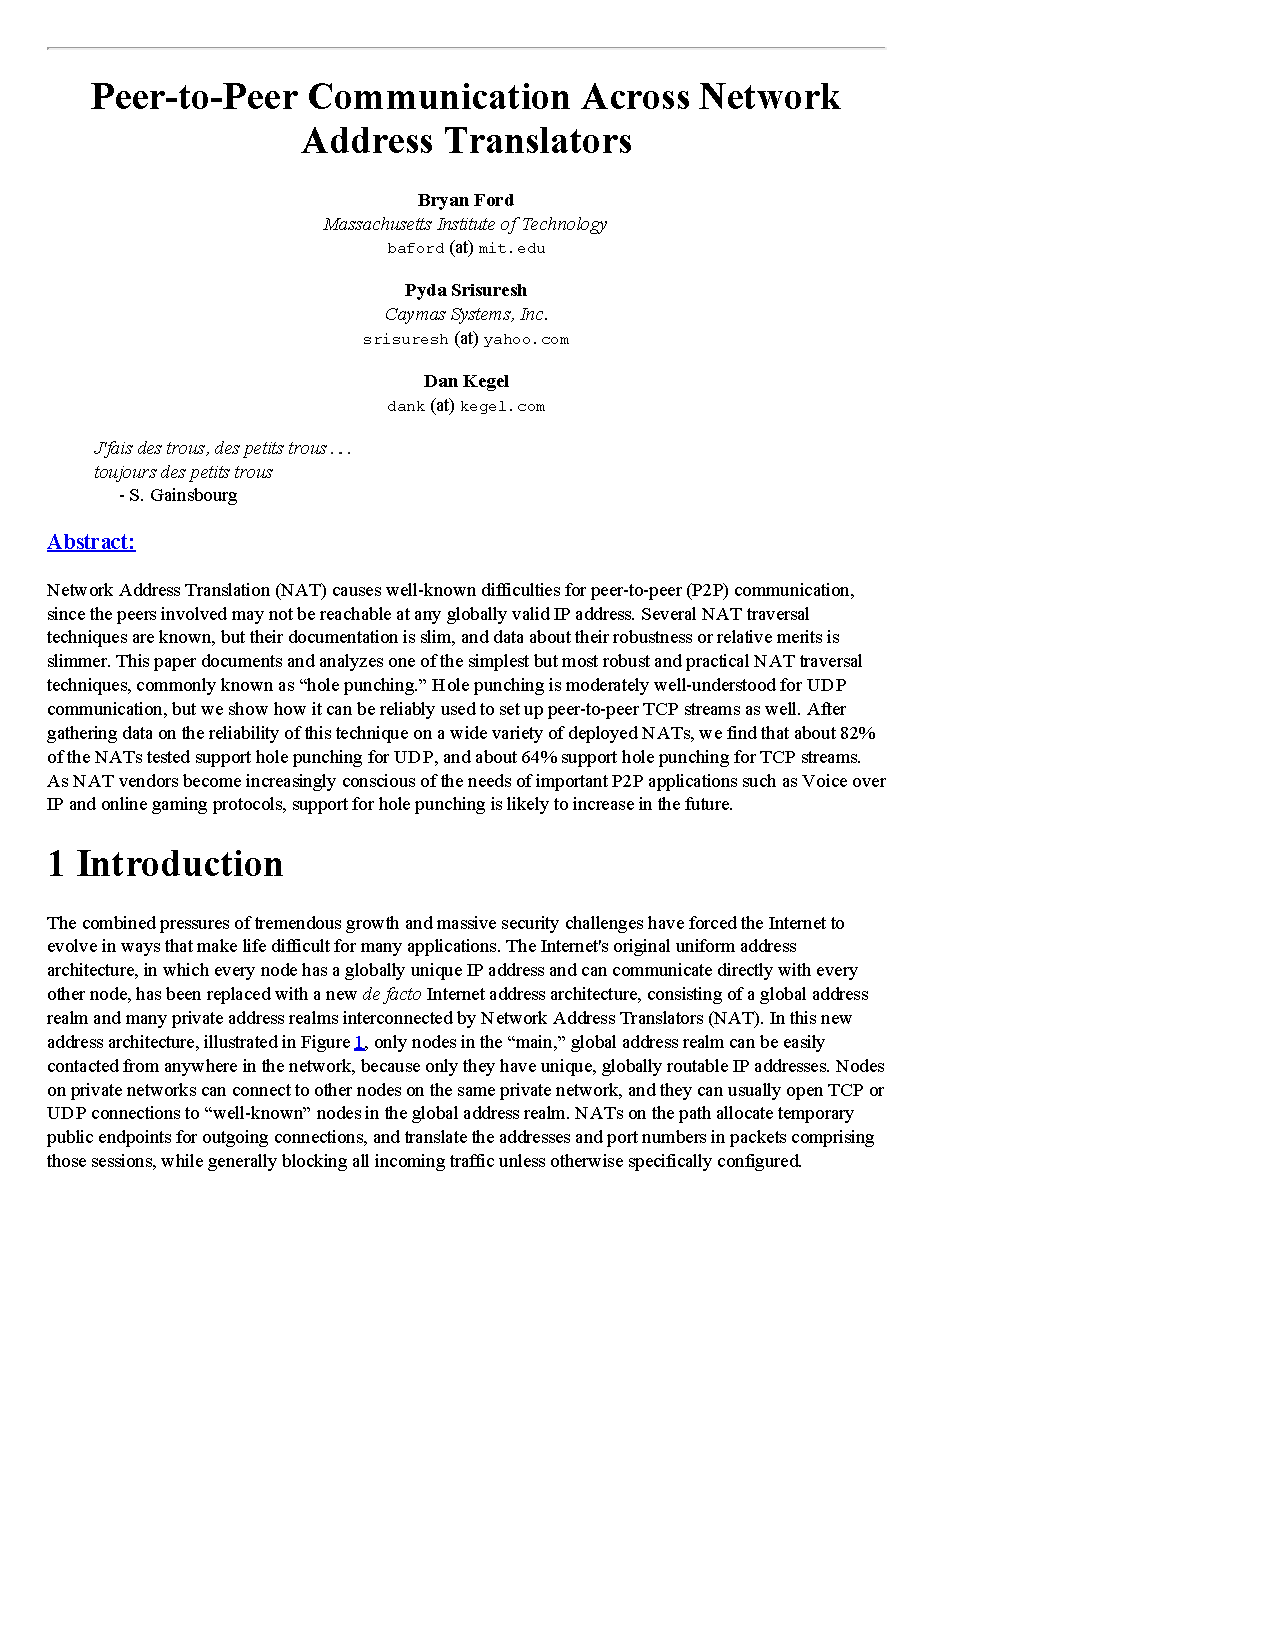
\includepdf[pages=-]{Ford}
\end{document}
